\documentclass{standalone}
\usepackage{tikz}

\begin{document}
	\tikzset{
	font=\footnotesize,
	minimum width=20
		}

	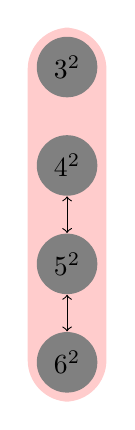
\begin{tikzpicture}
		\fill[color=red,opacity=0.2,rounded corners=15pt] (13,-3.25) rectangle (14,1.5);
		
		\node[shape=circle,fill=gray] (i) at (13.5,-2.75) {6$^2$};
		\node[shape=circle,fill=gray] (j) at (13.5,-1.5) {5$^2$};		
		\node[shape=circle,fill=gray] (k) at (13.5, -0.25) {4$^2$};
		\node[shape=circle,fill=gray] (l) at (13.5, 1) {3$^2$};
		\draw (i) edge[<->] (j) (j) edge[<->] (k);
	\end{tikzpicture}	
\end{document}  